\documentclass[conference]{IEEEtran}
\usepackage{graphicx}
\usepackage{tikz}
\usepackage{float}

 
\usepackage[colorlinks = true, citecolor = blue]{hyperref}

% math lib
\usepackage{amsmath}
\usepackage{mathrsfs}

% operators
\DeclareMathOperator*{\argmax}{arg\,max}
\DeclareMathOperator*{\argmin}{arg\,min}
\newcommand\ceiling[1]{\left\lceil #1 \right\rceil}

% empty set
\usepackage{amssymb}
\let\emptyset=\varnothing

% algorithms
\usepackage{algorithm}
\usepackage{algorithmic}
\renewcommand{\algorithmicrequire}{\textbf{Input:}}
\renewcommand{\algorithmicensure}{\textbf{Output:}}

\begin{document}
% --------------------------------------------
% --------------Change HERE! -----------------
% --------------------------------------------
\def\authorone{Akash Janardhan Srinivas}
\def\authortwo{Maanak Arora}
\def\groupid{5}
% --------------------------------------------
\title{CS258 Final Report: The RSA Problem}
\author{
    \IEEEauthorblockN{\authorone\ and \authortwo}
    \IEEEauthorblockA{
        Group \groupid
    }    
}

\maketitle
\IEEEpeerreviewmaketitle


\section{Methods: RL-based Routing}
\subsection{RL Algorithms}
% List RL algorithms and give a brief explanation of each
In this study we use two reinforcement learning algorithms - Proximal Policy Optimization (PPO) and Deep Q Network (DQN).

These algorithms have been implemented using Ray RLlib framework. PPO is a popular reinforcement learning algorithm that is known for its stability and efficiency. It updates the policy by iteratively improving it. It uses both policy gradient methods and trust region optimization. It alternates between sampling data through interaction with an environment and optimizing the surrogate objective function using stochastic gradient ascent.

DQN combines Q-learning with deep neural networks to handle high-dimensional sensory inputs. It was among the first successful applications of deep reinforcement learning. DQN uses experience replay to randomize data, thereby reducing the correlations between the observation sequence and smoothing changes in the data distribution. This also uses a target network to stabilize updates in learning.

The choice of these algorithms is due to their use in complex  decision-making tasks such as spectral slot allocation in optical networks. This is  suitable for  this research project.

\subsection{State Space}
% Explain state/action/reward
The state space done as a binary vector of the number of nodes in the network. It is represented as : self.observationSpace = spaces.Box(0, 1, shape=(len(self.graph.nodes),), dtype=np.float32).

Each part of this vector shows whether a node is part of the path currently involved in a spectral allocation. A value of '1' in the vector denotes the involvement of a node in the ongoing request, and '0' otherwise. This state space effectively captures the network status. It captures node engagement in requests, facilitating the agent's decision-making process.
% Make sure you provide enough information to reconstruct results
% Check https://gymnasium.farama.org/environments/box2d/lunar_lander/ for some examples

\subsection{Action Space}
The action space is a discrete set of possible choices, each corresponding to an edge in the graph: self.actionSpace = spaces.Discrete(len(self.graph.edges))

In this environment, an action represents selecting an edge of the graph to attempt the allocation of spectral slots for a communication request. The action space's size is determined by the number of edges in the network, allowing the RL agent to explore different paths for fulfilling the requests.

\subsection{Reward Function}
The reward function guides the RL agent's learning process.  It is designed to incentivize successful routing and penalize blocked requests. The reward structure is as follows:

Reward for successful routing: +1

Penalty for blocked request: -1

This reward function encourages the RL agent to find routes that minimize the number of blocked requests and maximize the successful delivery of data packets. By rewarding successful routing, the agent learns to identify and utilize available resources efficiently. The penalty for blocked requests discourages the agent from selecting congested paths. This promotes picking of routes.

\subsection{Starting state}
The starting state for each episode is the initial configuration of the network, where no requests have been processed, and all resources (spectrum slots) are available. The initial request is generated with a random source and destination pair, as well as a randomly determined holding time within the specified range.

\subsection{Episode termination}
An episode terminates when:

All requests have been processed: The episode finishes after accepting (or blocking) the last request. There is no need to wait for all residing requests to leave. We only care about the utilization until the handling of the last request.

Maximum steps reached: The episode terminates if the maximum number of steps, corresponding to the number of requests, has been reached.

\subsection{Arguments}
To configure the environment, the following arguments can be specified:

topology file: The path to the GML file containing the network topology.

capacity: The capacity of each link in the network, representing the number of spectrum slots available.

num requests: The number of requests to be processed in each episode.

min ht: The minimum holding time for a request.

max ht: The maximum holding time for a request.

\section{Method: Spectrum Allocation}
% Explain your heuristic
% If you have multiple, you can make subsections 

The algorithm attempts to find the shortest path for each request and allocate a spectral slot that is available across all edges on this path. If successful, the request is accommodated; otherwise, it is considered blocked. This method focuses on maximizing the utilization of network resources while minimizing the blocking of requests.
\newline

Spectrum Allocation Heuristics:

Request Processing - he algorithm calculates the shortest path from the source to the destination node using Dijkstra's algorithm, facilitated by the NetworkX library.

Slot Availability - The algorithm checks for available spectral slots on each edge of the identified path. An available slot is one that is not currently allocated to any other request, or if allocated, will be freed up before the current request's health time expires.

Alocation - If there exists at least one common spectral slot across all edges of the path, the algorithm allocates this slot to the request across all these edges. The spectral slot is then marked as occupied for the duration of the request's health time. If no common slots are available, the request is blocked, indicating a failure to allocate the necessary resources.
As time progresses, the health time of active requests in each spectral slot is decremented. Once a request's health time reaches zero, the spectral slot is freed up, making it available for future requests.

% If you borrow some ideas from papers, cite them with bibtex (e.g. \cite{8509143})


\section{Results}
\subsection{Learning Curve}
% Insert figures
% Explain the results

The learning curves depicted in the figures demonstrate the performance progression of both the Proximal Policy Optimization (PPO) and Deep Q-Network (DQN) algorithms across two distinct cases in our spectrum allocation simulation.

\begin{figure}[H]
    \centering
    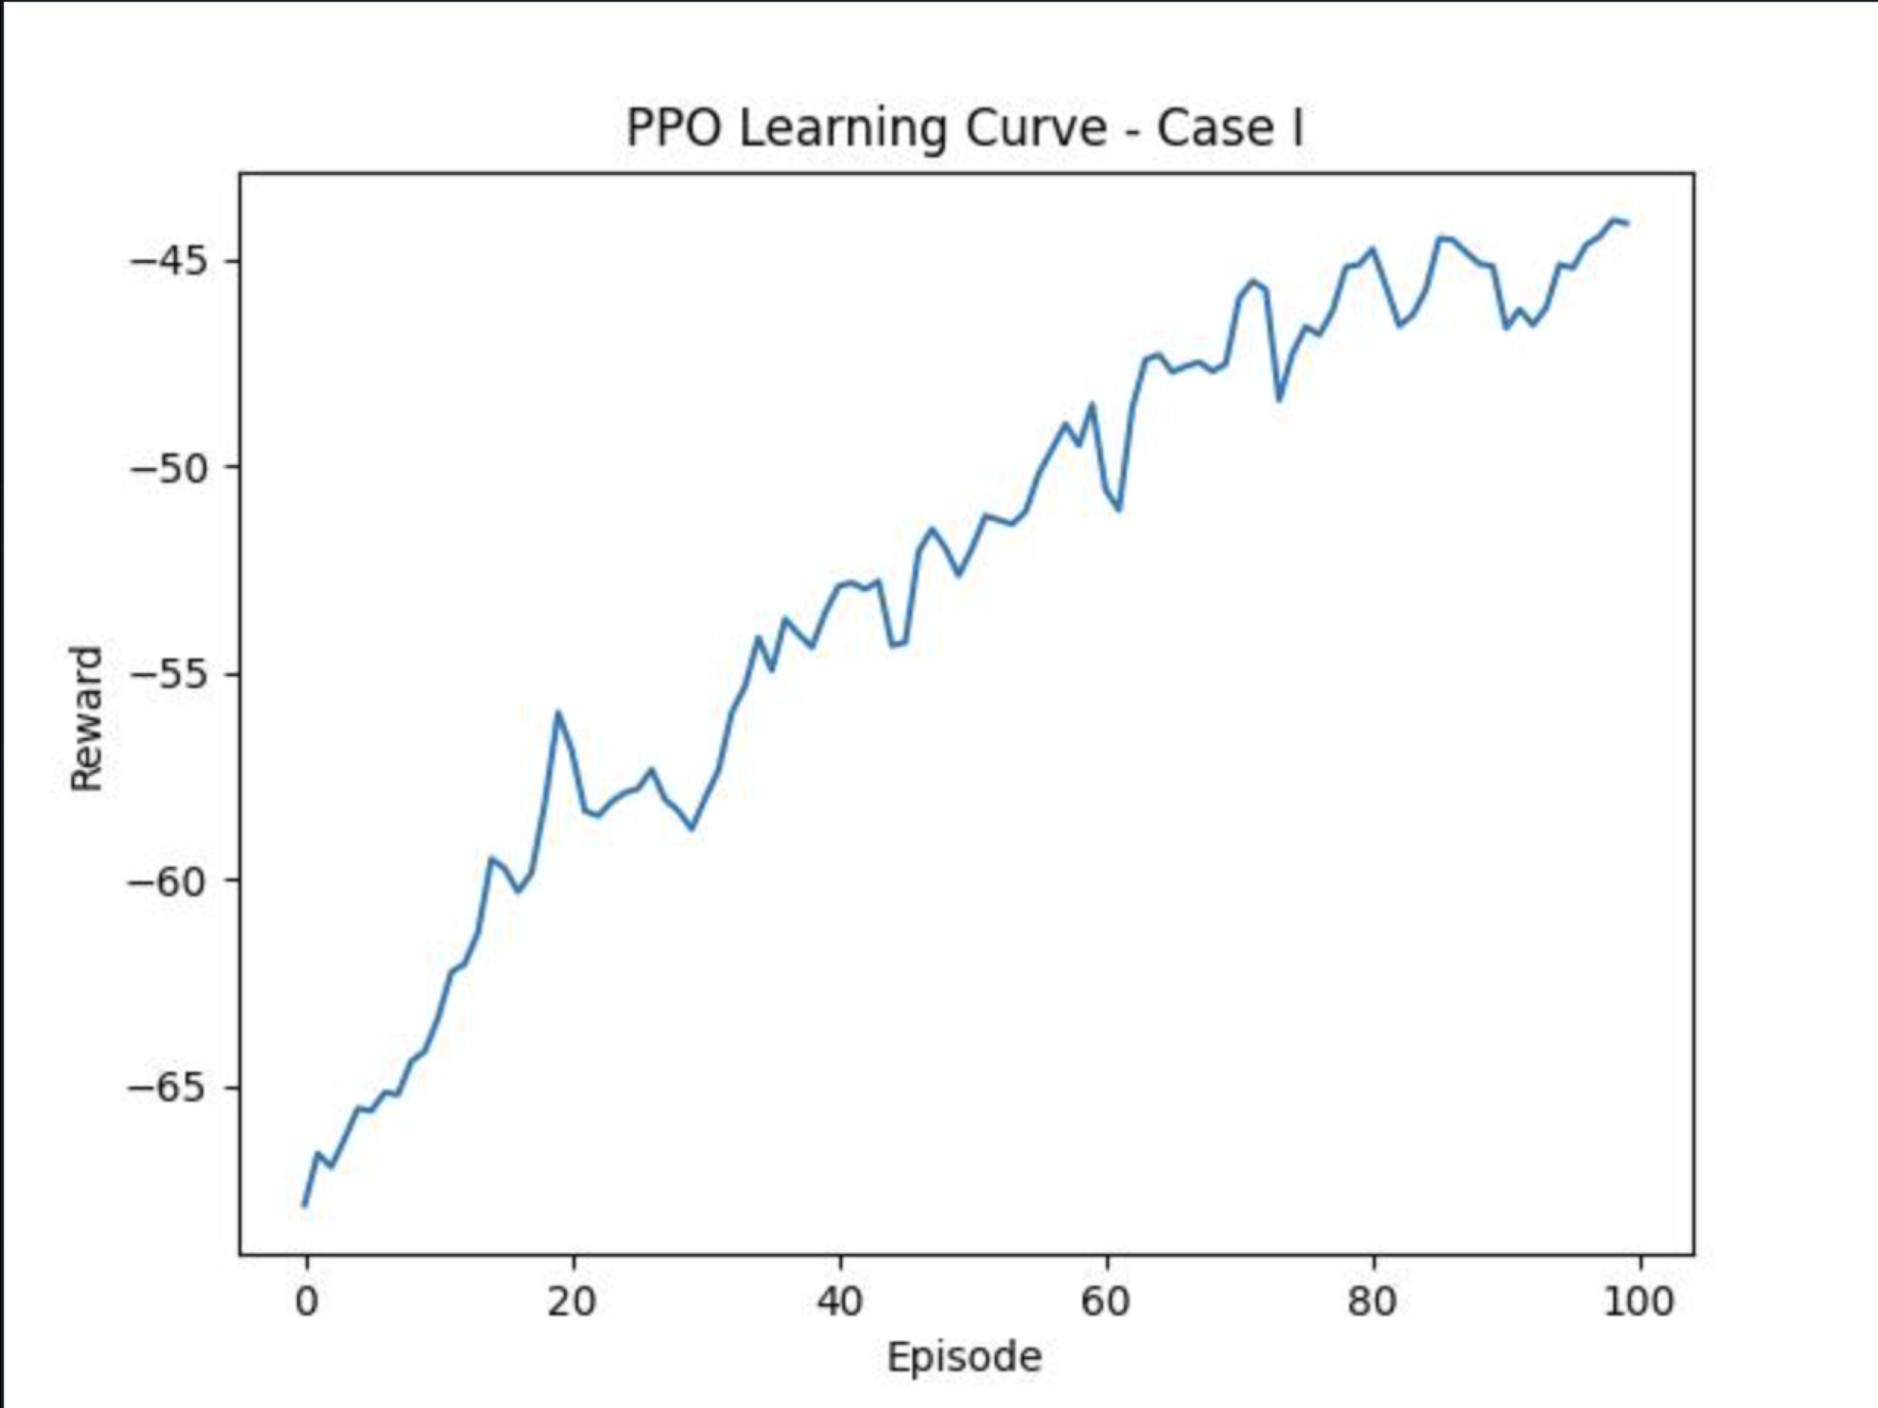
\includegraphics[width=0.5\linewidth]{Fig 1.png}
    \caption{PPO Learning curve Case 1}
    \label{fig:enter-label}
\end{figure}

Figure 1 shows the PPO Learning Curve for Case I, where the reward steadily increases, indicating a successful learning and adaptation process by the agent in maximizing the successful allocation of spectral slots over episodes. The positive trend suggests that the agent becomes more proficient at handling the given scenarios in this particular case, which is characterized by a specific pattern or distribution of network requests.

\begin{figure} [H]
    \centering
    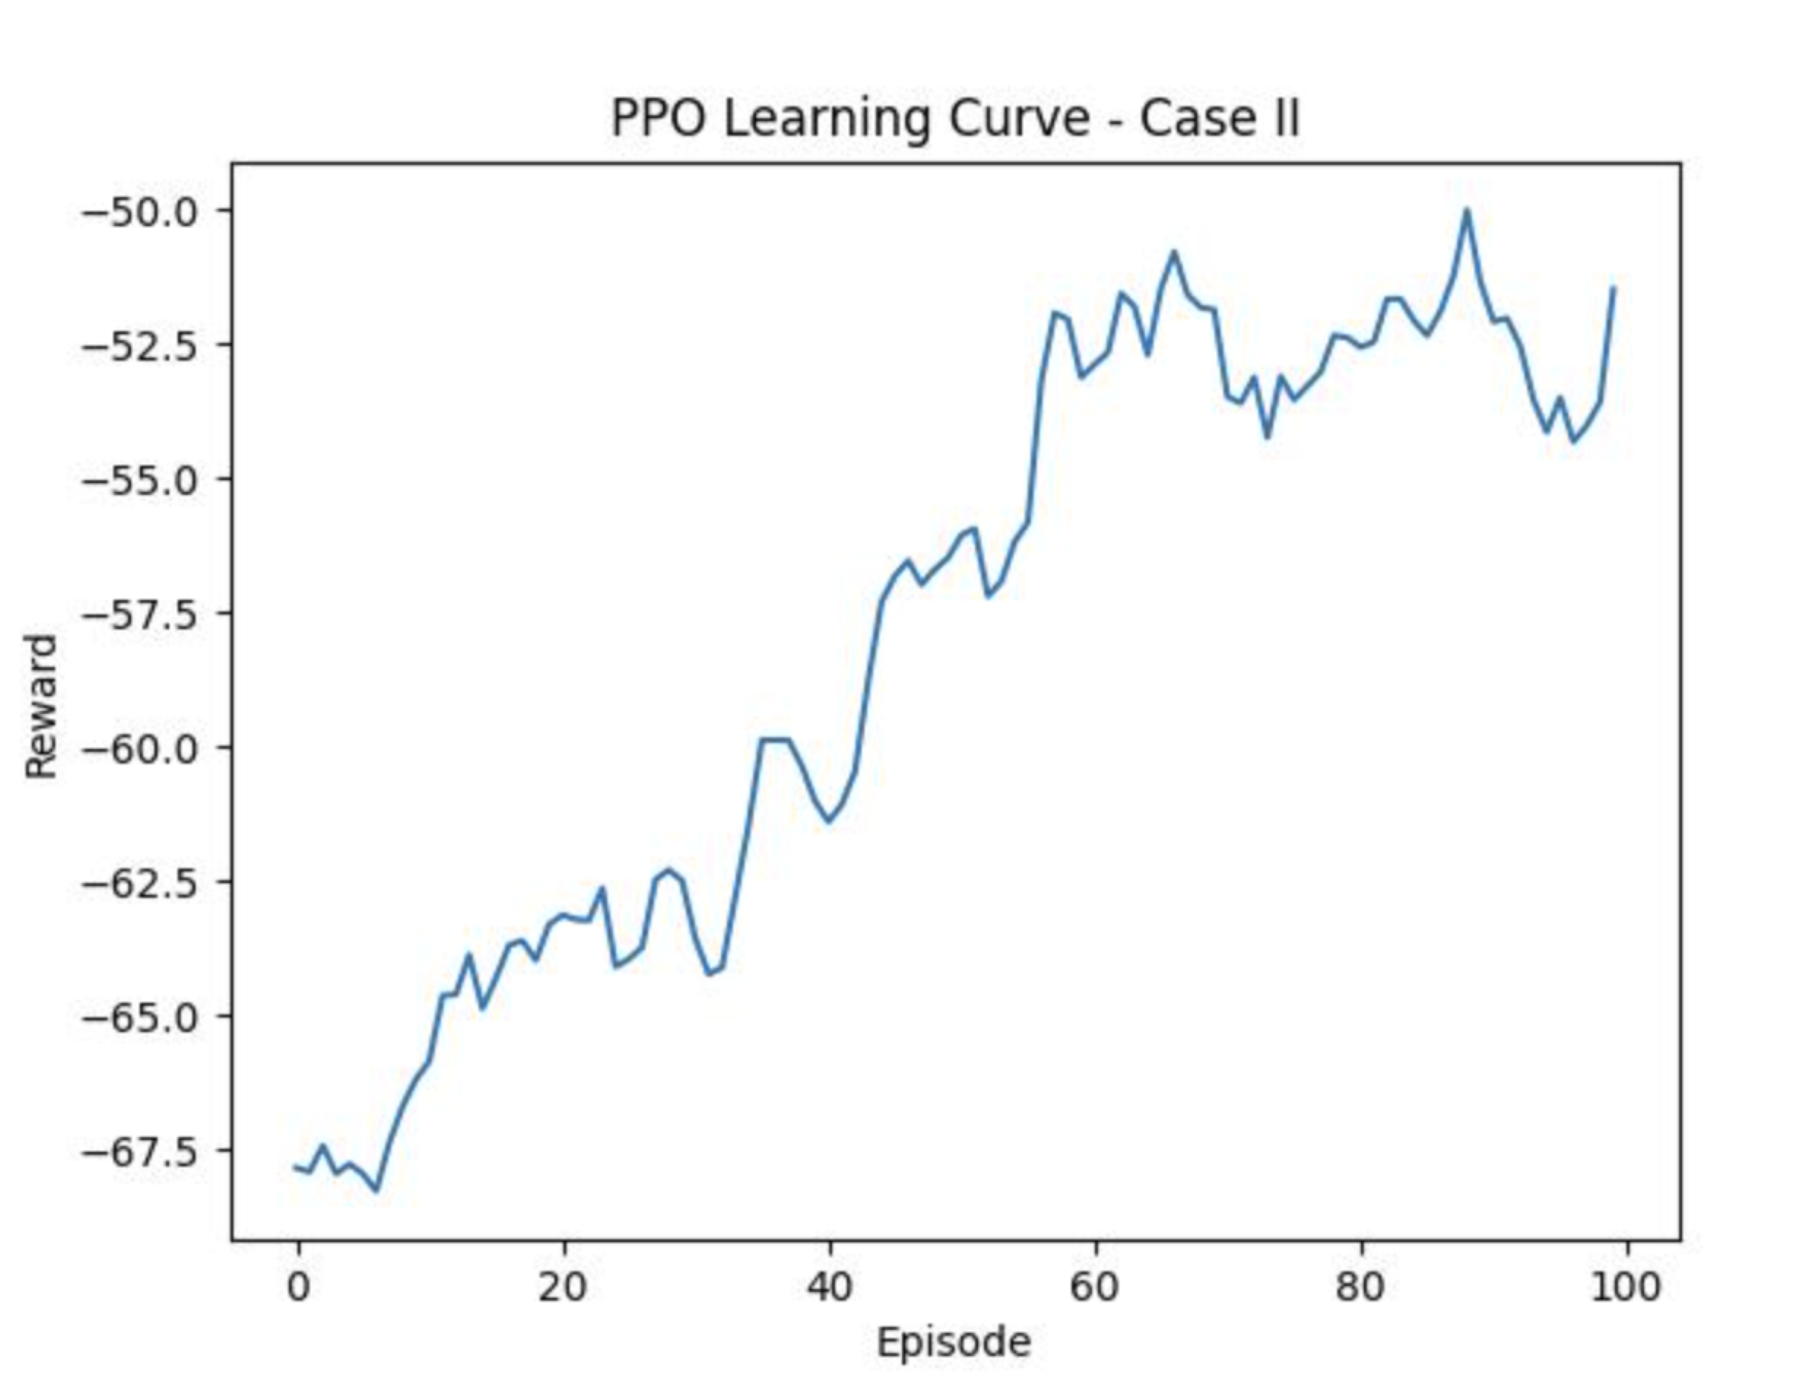
\includegraphics[width=0.5\linewidth]{Fig 2.png}
    \caption{PPO Learning curve Case 2}
    \label{fig:enter-label}
\end{figure}

Figure 2 presents the PPO Learning Curve for Case II, characterized by a more fluctuating yet generally positive trend. This indicates variability in the scenario or an increased complexity in the environment which the PPO agent is gradually adapting to.

\begin{figure} [H]
    \centering
    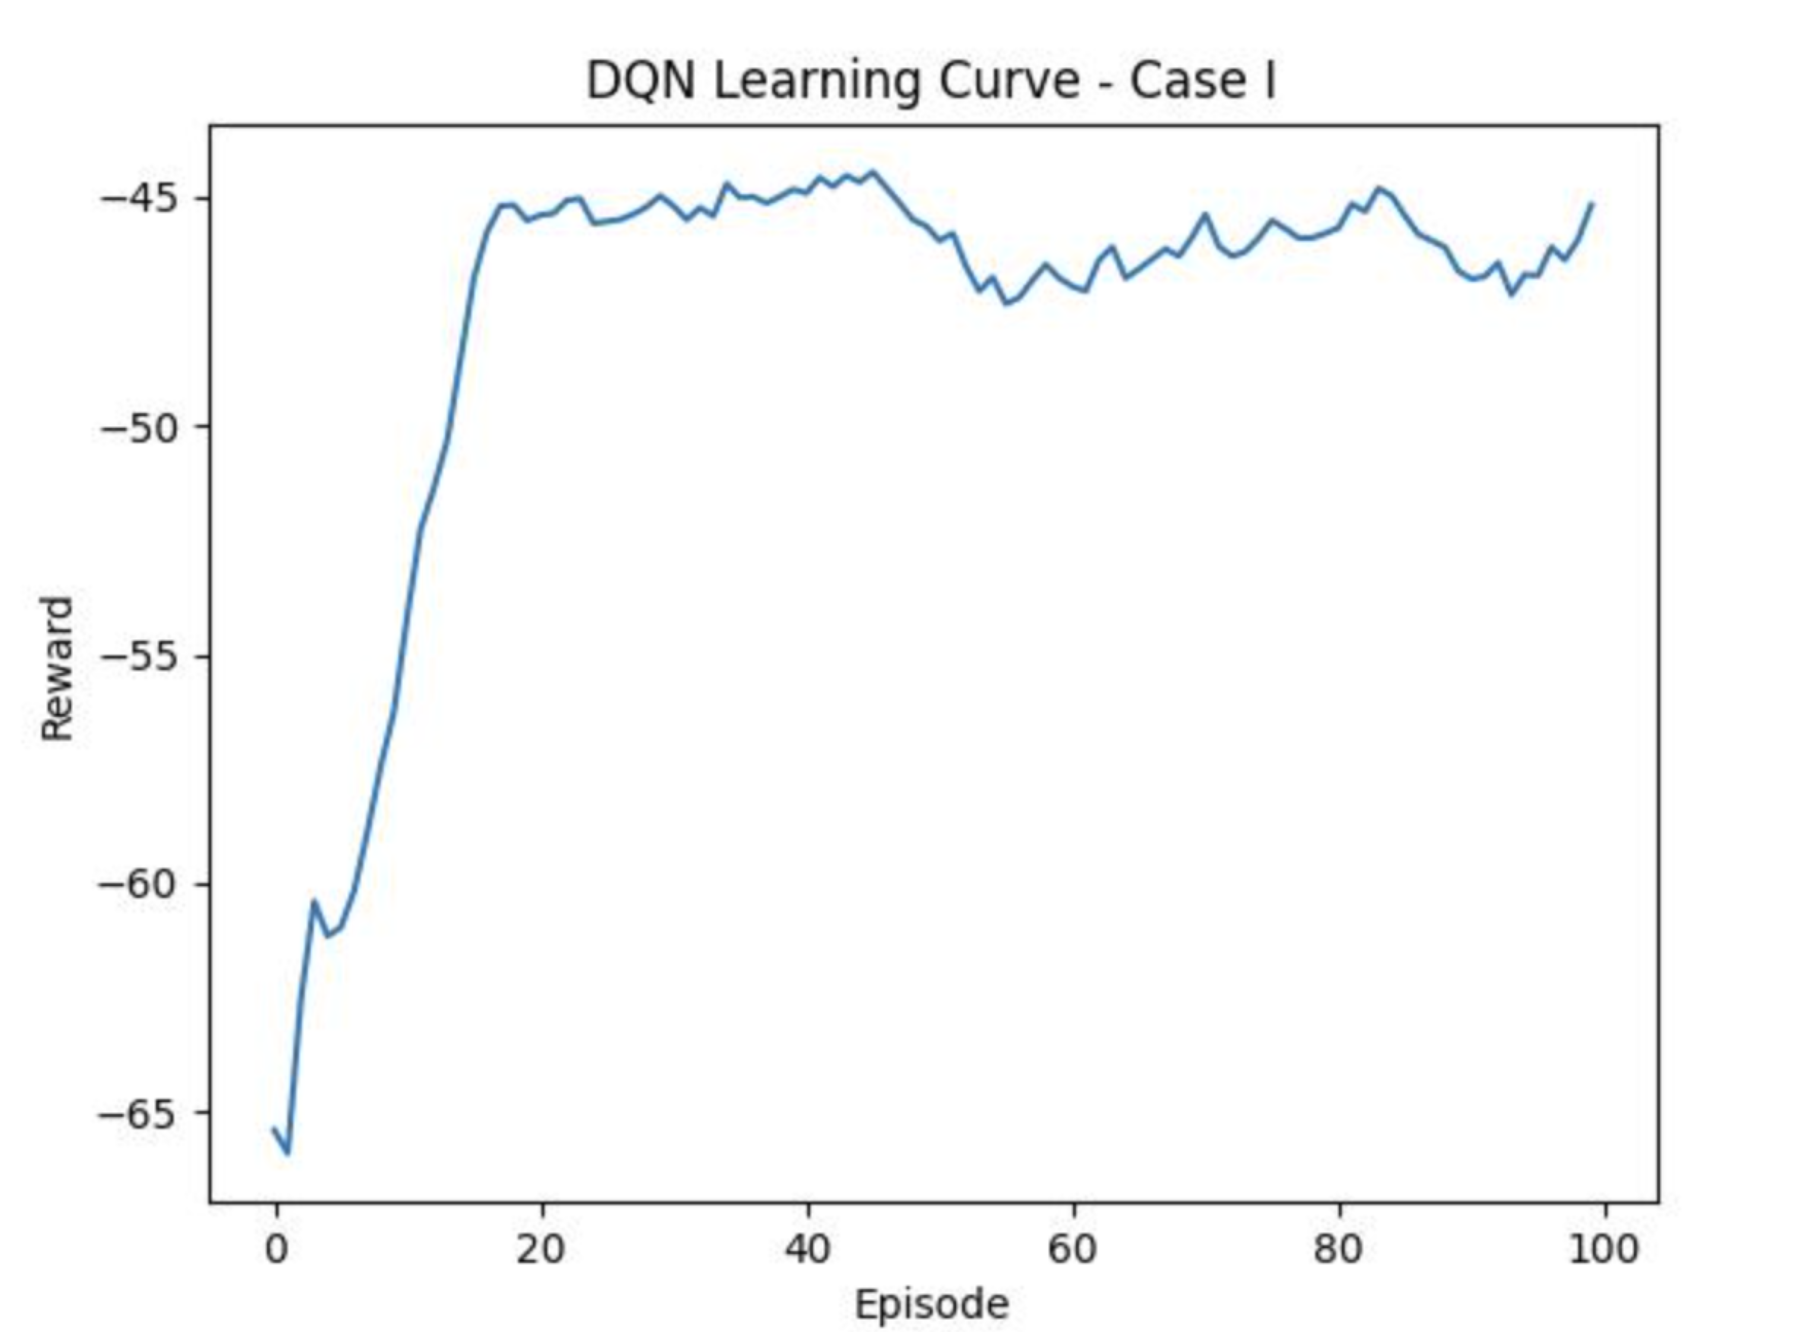
\includegraphics[width=0.5\linewidth]{Fig 3.png}
    \caption{DQN Learning curve Case 1}
    \label{fig:enter-label}
\end{figure}

\begin{figure} [H]
    \centering
    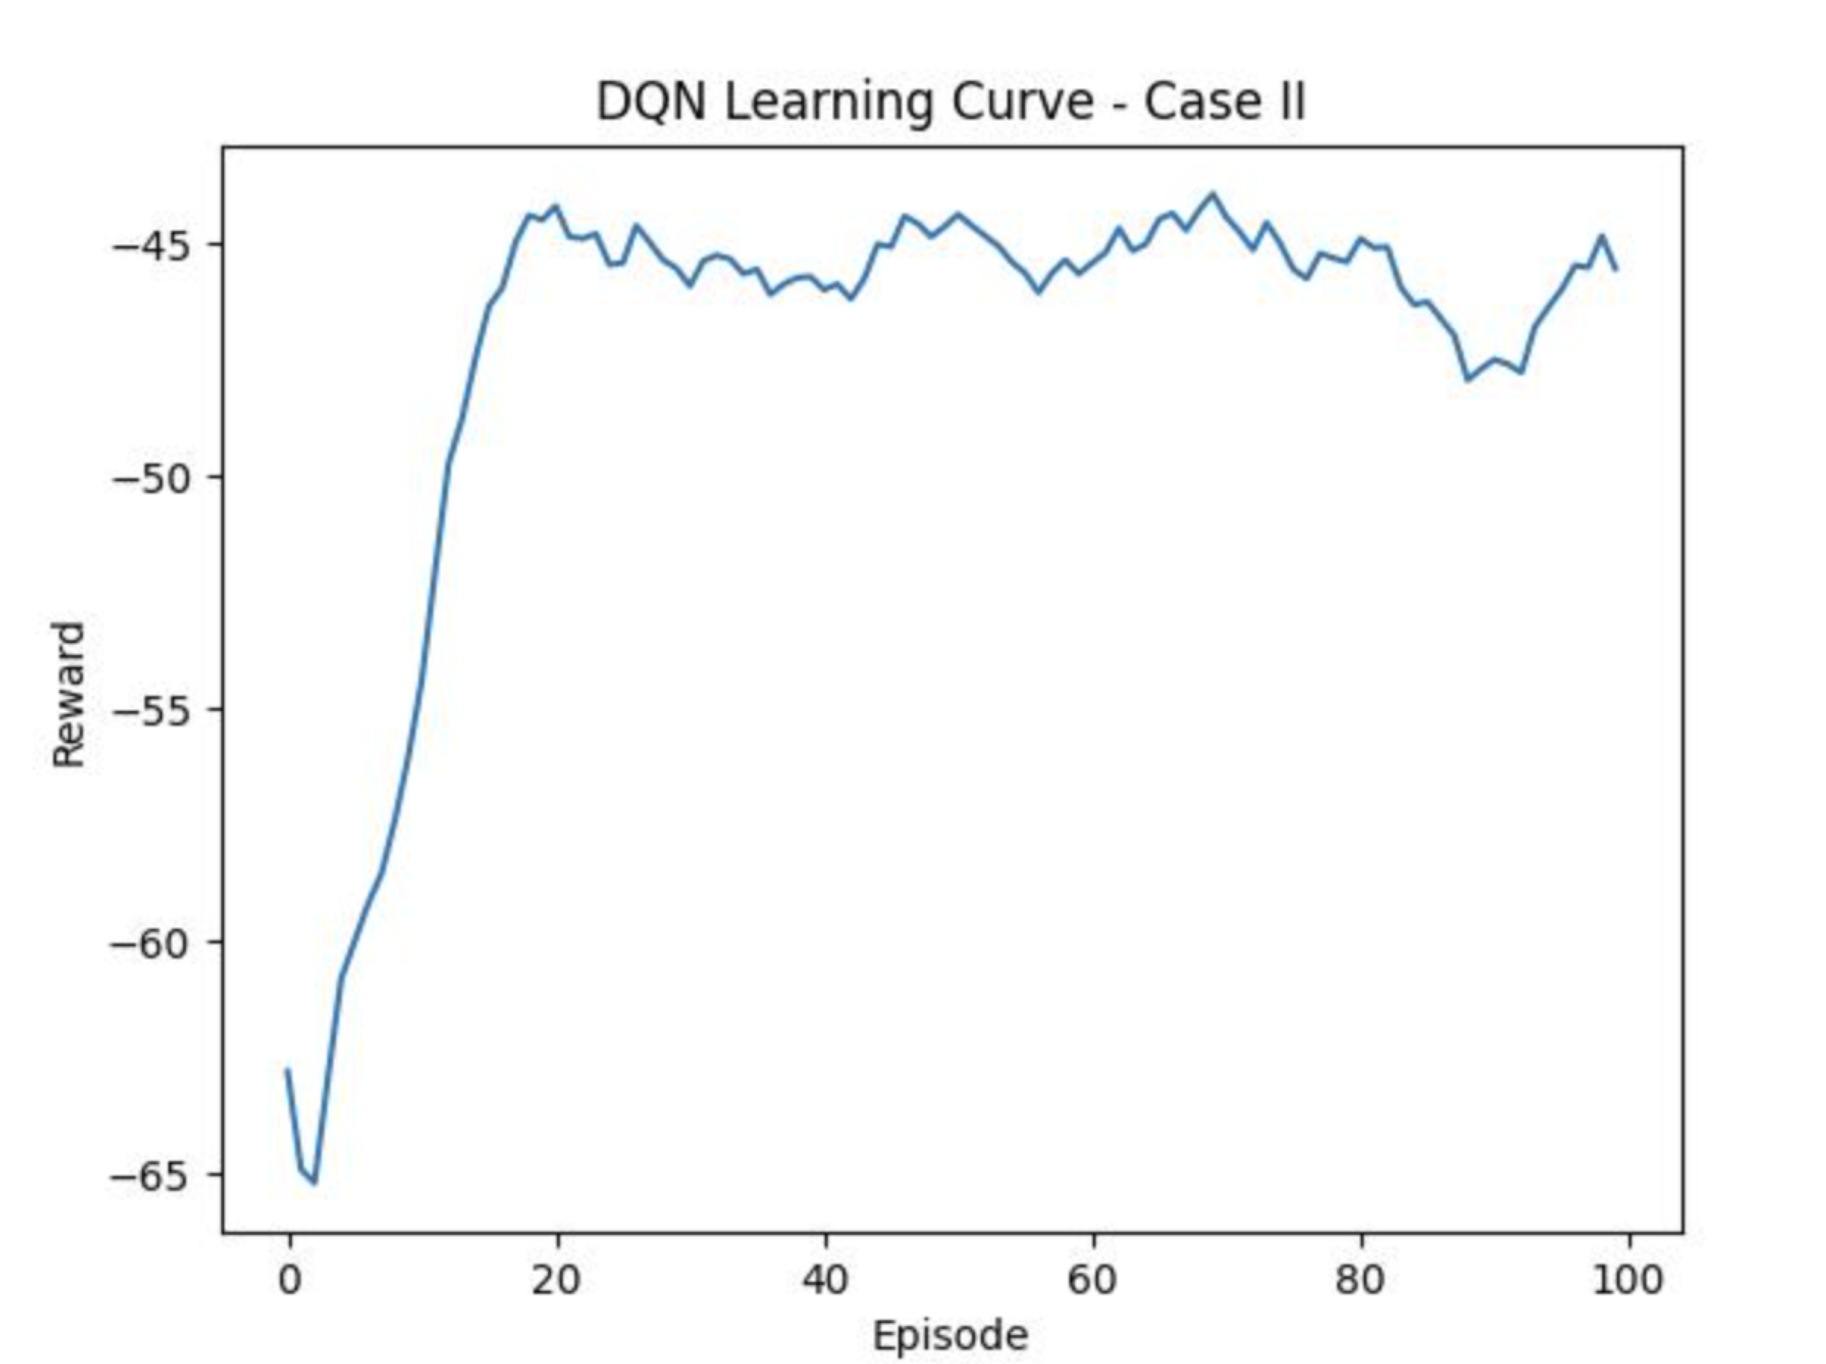
\includegraphics[width=0.5\linewidth]{Fig 4.png}
    \caption{DQN Learning curve Case 2}
    \label{fig:enter-label}
\end{figure}

Figure 3 and Figure 4 show the DQN Learning Curves for Cases I and II, respectively. In both cases, the DQN algorithm demonstrates an initial sharp increase in reward, followed by stabilization. This pattern suggests that DQN quickly learns effective strategies for spectral allocation but then faces challenges in further optimizing or improving beyond a certain point due to the constraints or complexities of the environment.

\subsection{Utilization (The Objective)}
The primary objective of employing reinforcement learning in this optical network environment is to optimize the utilization of spectral slots to reduce the number of blocked requests effectively. The gradual increase in rewards observed in the learning curves correlates with improved utilization rates. Higher rewards signify fewer blocked requests and better overall network resource management. This outcome directly aligns with the goal of enhancing spectral efficiency.

\subsection{Comparison}
Comparison of the performance of PPO and DQN over both cases reveals key differences in learning capability and efficiency.

Proximal Policy Optimization (PPO):

Case I: PPO demonstrates a smooth and steady improvement in rewards, showing its capability of gradual learning and adaptation to the environment. The consistency of the learning pattern suggests that PPO will be highly suitable for situations where long-term learning stability is a highly desired feature of the learning algorithm.
Case II: In Case II, the learning curve of PPO indicates the same pattern, improving with the increase in time. The rewards indicate the strength of PPO in environments where sustained learning and adaptation are highly required.

Deep Q-Network (DQN):

Case I: DQN shows a steep initial increase in rewards and then starts to level off at a high reward plateau. This indicates DQN is very good at identifying quickly successful strategies for the given environment, thus being very suitable for environments where a solution is highly beneficial to be found quickly. However, the plateau indicates that this method might have difficulty improving the performance even further than the initial gain.
Case II: In Case II, DQN depicts the same pattern of a steep initial rise in reward; however, there are some fluctuations. This fluctuation indicates the problems of DQN in maintaining stability over a longer period.
Heuristic Algorithm:

This heuristic-based spectrum allocation algorithm serves as a baseline for comparison. Even though it is much simpler and less adaptive than the RL methods, still it sheds light on the efficiency of resource utilization in a very simple way.
Comparison of Network Utilization: Comparing the network utilization of both PPO and DQN, they outperform the heuristic algorithm by showing a higher utilization percentage. In PPO, the performance is consistent, which ensures stable utilization, whereas in DQN, the initial good performance offers high utilization very fast but also with some fluctuations.


\bibliography{ref}
\bibliographystyle{ieeetr}
[1] Schulman, J., Wolski, F., Dhariwal, P., Radford, A., & Klimov, O. (2017). Proximal Policy Optimization Algorithms. ArXiv. /abs/1707.06347

[2] Cassady, Caleb, "Reinforcement Learning with Deep Q-Networks" (2022). Masters Theses & Specialist Projects. Paper 3554.
https://digitalcommons.wku.edu/theses/3554

\end{document}



